% !TeX spellcheck = hu_HU
% !TeX encoding = UTF-8
% !TeX program = xelatex
%----------------------------------------------------------------------------
\section{Állapotgép leíró nyelv}\label{sec:uses:fsm}
%----------------------------------------------------------------------------

A sokak által ismert és egyszerű véges állapotgépek \gls{FSM} leírására adott szakterület-specifikus nyelv jó példa tud lenni egy \gls{DSL} készítésére képes eszköz számára.
Ez többek között azért van, mert ezeket a matematikai jellegű struktúrákat egy deklaratív, letisztult, egyszerű nyelvben is le lehet írni szépen és elegánsan.
Ez kifejezetten egy előnye egy \gls{DSL}-nek, míg egy általános célú nyelvben ezt gyakran jóval bonyolultabban lehet megvalósítani.
Ebben a szekcióban, az előzőeknek megfelelően, én is megadok egy \gls{FSM} megvalósítást, amelyikkel egyszerű véges automatákat lehetséges megvalósítani.
A konkrét megvalósító C4 kód % todo ref
függelékben, egy példaként megvalósított állapotgép látható \aref{fig:ex-stm}.~ábrán. A \gls{DSL}-ben írt kód a pedig alább következik \aref{lst:ex-fsm}.~listázásban.

\begin{figure}[hbt]
	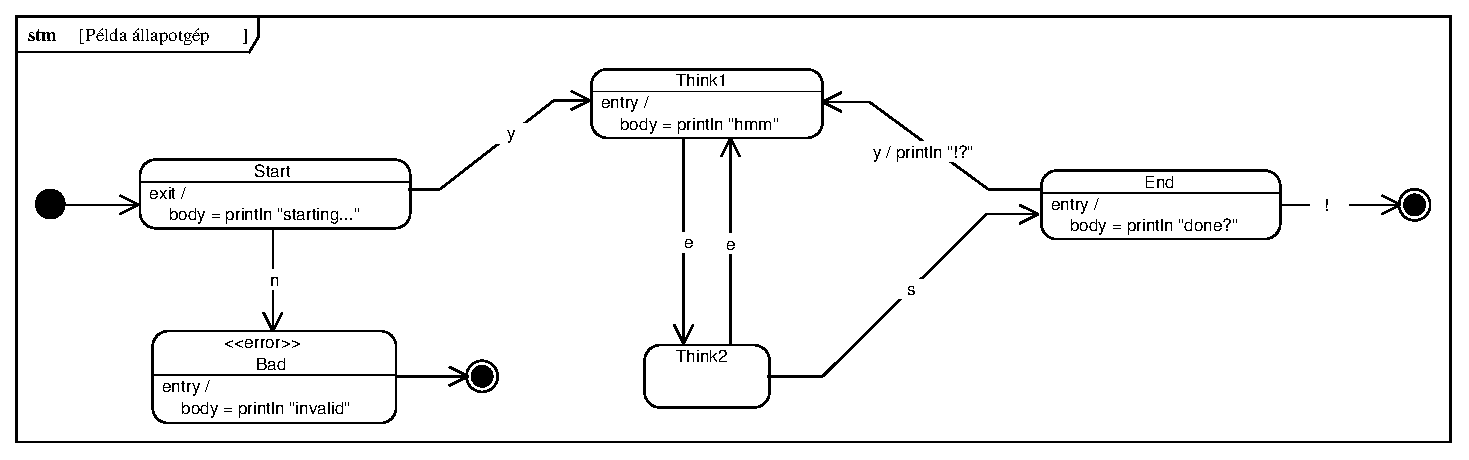
\includegraphics[width=\linewidth]{content/ex-stm.eps}
	\caption{A megvalósított állapotgép}\label{fig:ex-stm}
\end{figure}

\begin{lstlisting}[gobble=2,numbers=left,caption={C4 állapotgép \gls{DSL} használati példa},label=lst:ex-fsm]
	let myfsm fsm
		start state "start"
			leave { println "starting..." }

		final state "done"

		error state "bad"
			enter { println "invalid" }

		state "think1"
			enter { println "hmm" }

		state "think2"

		state "end"
			enter { println "done?" }

		on "n" from "start" to "bad"
		on "y" from "start" to "think1"

		on "e" from "think1" to "think2"

		on "e" from "think2" to "think1"
		on "s" from "think2" to "end"

		on "y" from "end" to "think1"
			do { println "!?" }
		on "!" from "end" to "done"
	done
\end{lstlisting}

Ami a C4 előnye ebben az esetben, más nyelvleíró eszközökkel szemben, hogy a megvalósítás során a megfelelő szemantikát is tudjuk, ugyanabban a nyelvben definiálni.
Ezzel ennek az állapotgépnek a futtatása, amelyik a {\tt myfsm} változóban található, egy olyan léptető függvény definiálásával megvalósítható egy lépése, amelyik átveszi a jelenlegi állapotgép állapotot, lépteti egy bemenetnek megfelelően, majd visszaadja az új állapotot -- a közben szükséges akciókat végrehajtva.
Ennek a lépés függvénynek ismételt hívásával pedig tetszőleges sok lépést lehetséges léptetni a rendszer állapotán.

A léptető függvény megvalósítása erősen függ az állapotgép leíró belső megvalósításától, az általam adott szintén megtalálható a függelékben {\tt fsm\_step} néven, míg az üres sorig olvasó ciklikusan léptető függvény a {\tt step\_until\_empty}.
Utóbbi beolvas egy sort, és ha az üres kilép, különben a bemenetet továbbítja a léptető függvénynek, majd rekurzióba kezd.
Ezeket ismerve az alábbi kódrészlettel futtathatóvá válik a {\tt myfsm} változóban tárolt állapotgép.

\begin{lstlisting}[gobble=2,numbers=left]
	step_until_empty myfsm
\end{lstlisting}

\todo[inline]{Szar az egész}

Láthatólag ez egy rövid kódrészlet, az alapvetően egyszerű trükkök mind el vannak rejtve a \gls{DSL} megvalósítása mögé, így az állapotgépet használónak csak azzal kell foglalkoznia, amivel szeretne.

























